\chapter{Experiments}\label{C:experiments}

\section{Introduction}

All the algorithms above excluding DQN can work on continuous action spaces. This makes them suited for continuous control tasks that are common within the robotic control domain. I will conduct experiments using the Gymnasium \cite{towers2024gymnasium} library which provides a framework to use among other things some Mujoco \cite{todorov2012mujoco} environments. Specifically I will use \texttt{Ant-v5, Humanoid-v5, Pusher-v5, HalfCheetah-v5, HumanoidStandup-v5, Swimmer-v5, Hopper-v5, InvertedDoublePendulum-v5, Walker2d-v5} and \texttt{Hopper-v5} which cover a range of locomotion tasks. I will run the experiments we have looked at above on theses environments to understand how well they learn.

There are many different dimensions in which we can judge the learning performance of an algorithm. The most common and useful ones are general across not continuous control problem but all reinforcement learning problems. These common and overarching dimensions are:

\begin{itemize}
    \item Sample efficiency: How many environment interactions does it take to learn a task?
    \item Computational efficiency: How much computation does it take to learn a task?
    \item Stability: How stable is the learning process?
    \item Asymptotic performance: What is the maximum performance of the algorithm?
    \item Generalization: How well does the algorithm generalise to new tasks, be it new environments or agent?
\end{itemize}

\section{Baseline Experiments}

I will look at two things for all of my baseline algorithms. The first is the sample efficiency and the second is the computational efficiency. It is important to understand both of these metrics as it can sometimes be easier to trade computational efficiency for sample efficiency. Therefore to make a true improvment to a model it must be better at either/both of these metrics will not reducing the other metric.

\subsection{Sample Efficiency}
To measure the sample efficient I will look at the average reward over 10 episodes every 1000 steps. This will give a learning curve to demonstrate how effective its actions are given how many interactions it has had with the environments.

\begin{figure}[H]
    \centering
    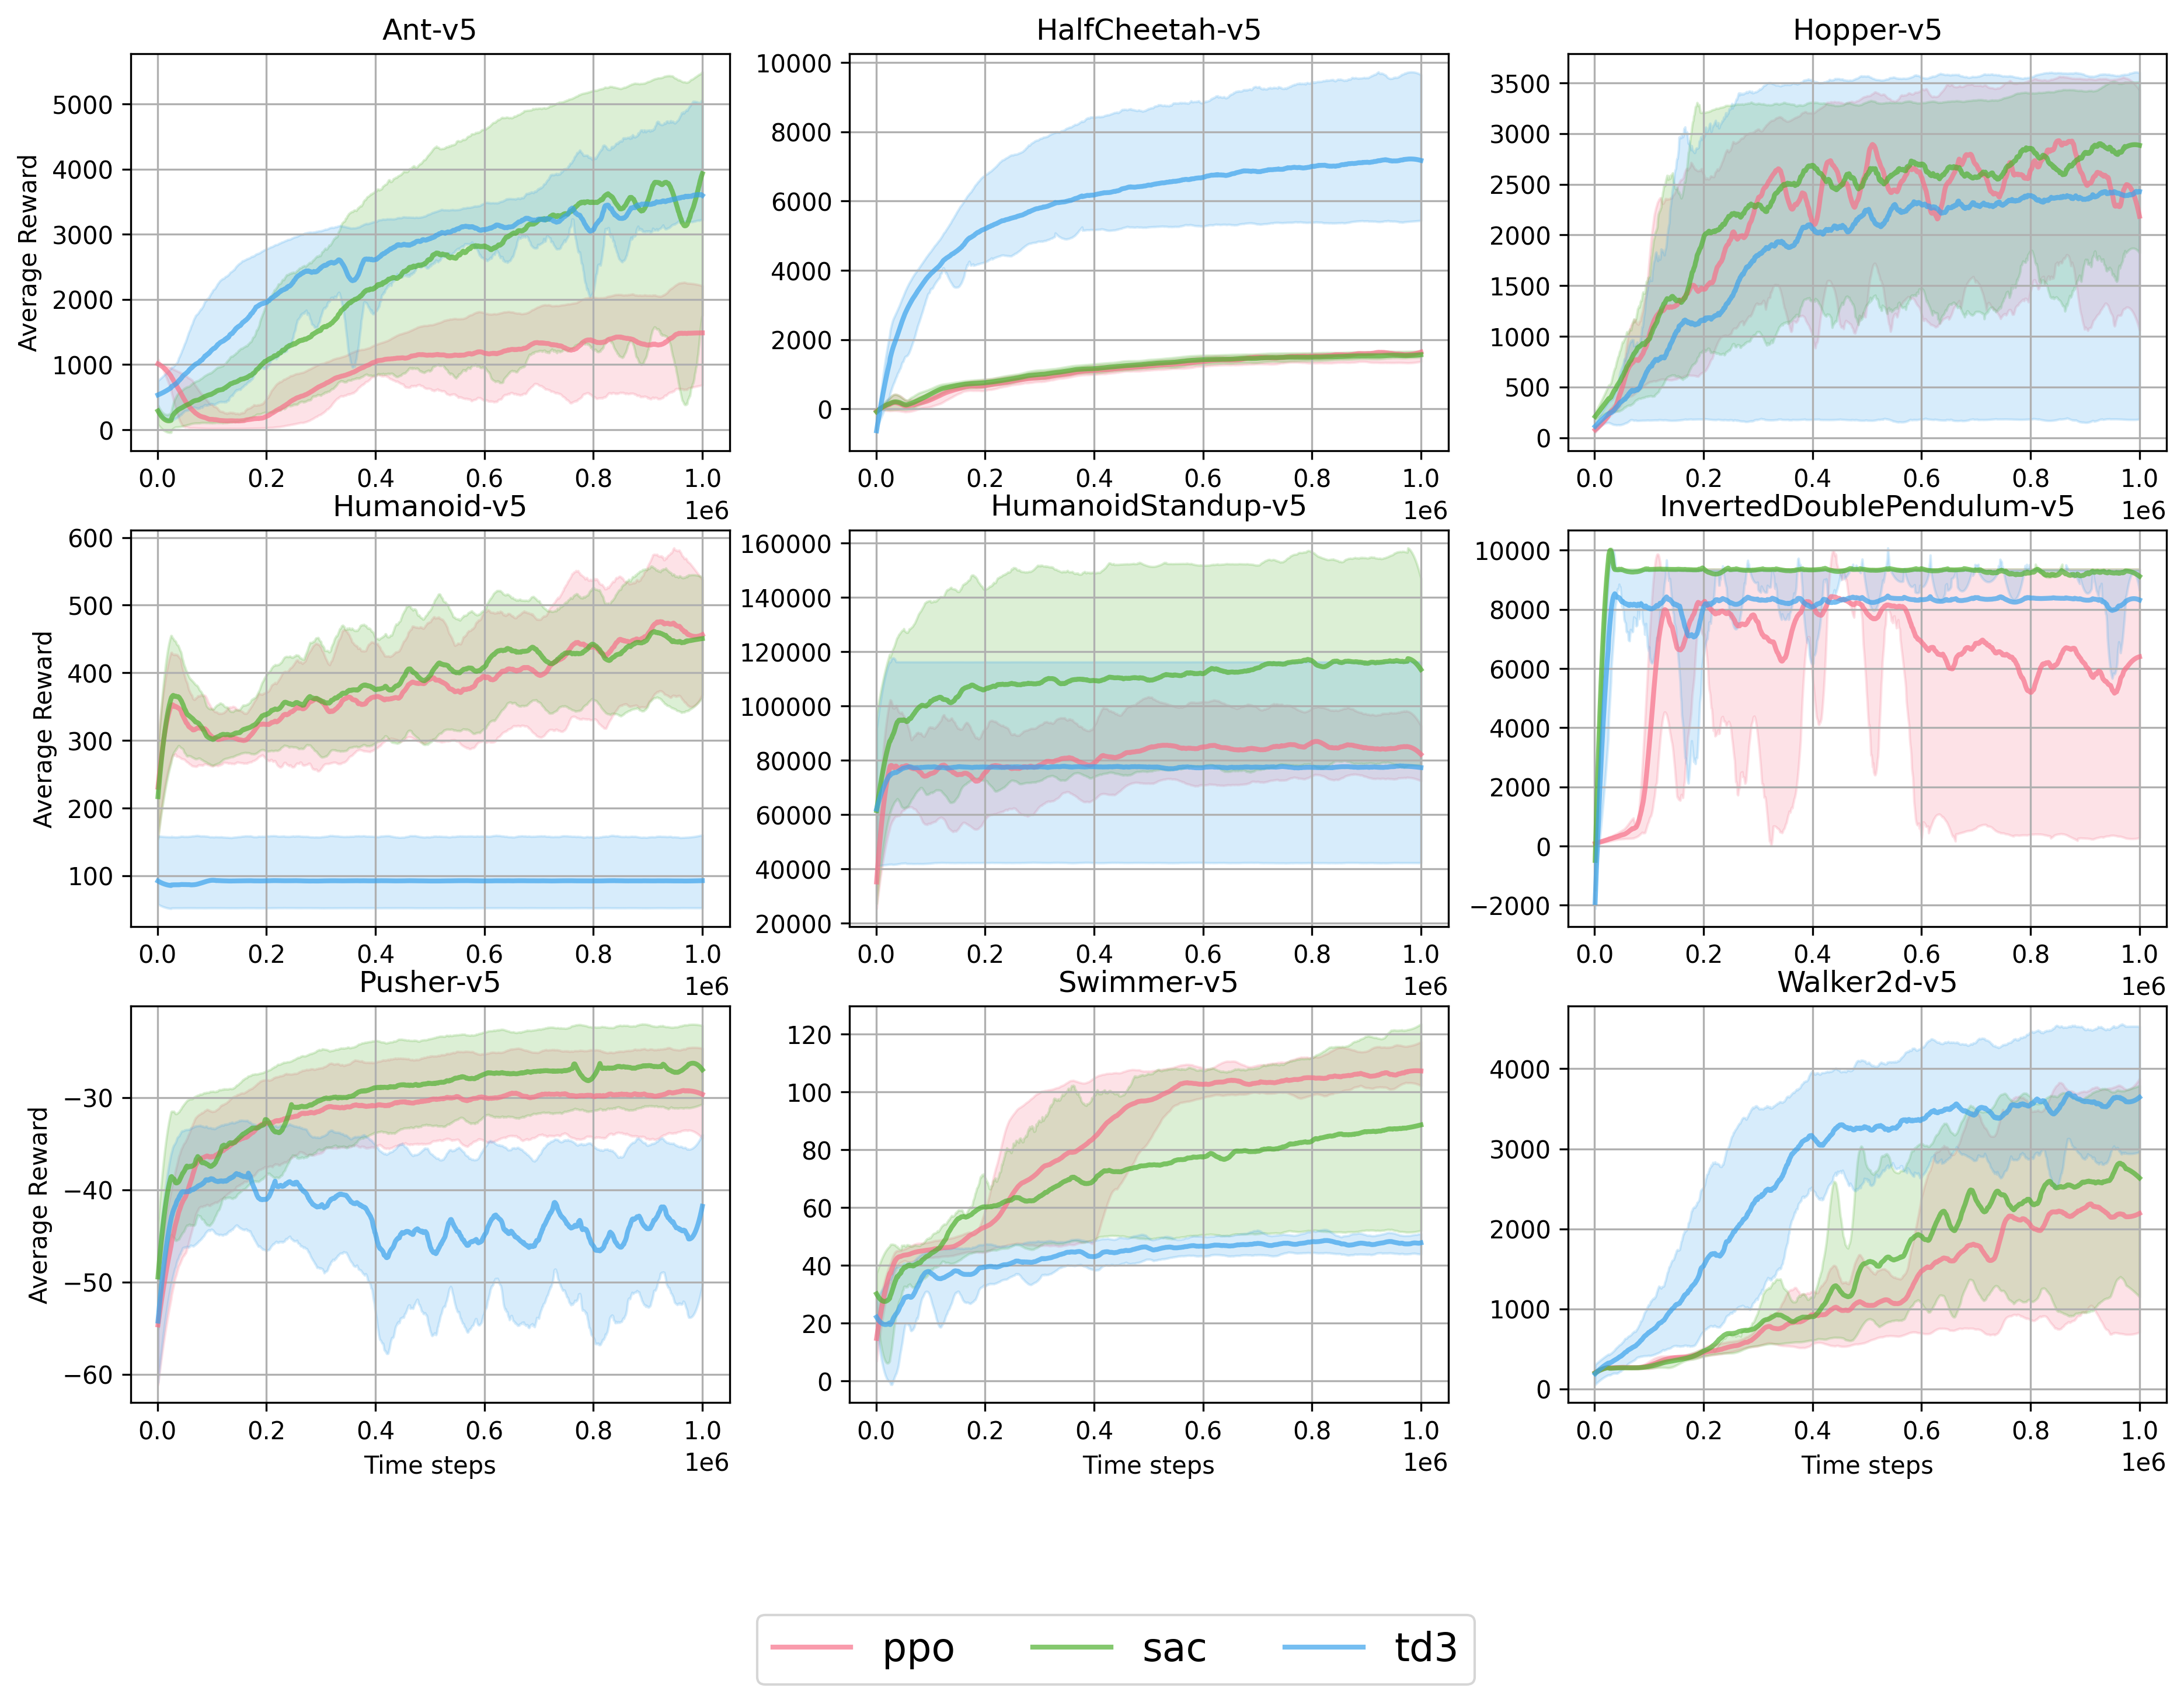
\includegraphics[width=\textwidth]{figures/baseline_results.png}
    \caption{Sample Efficiency of older algorithms. The line is a smoothed average return across the 100 episodes made by each seed every 1000 times steps. The shaded area is a smoothed 70\% confidence interval highlighted}
    \label{fig:sample_efficiency_baseline}
\end{figure}

\begin{figure}[H]
    \centering
    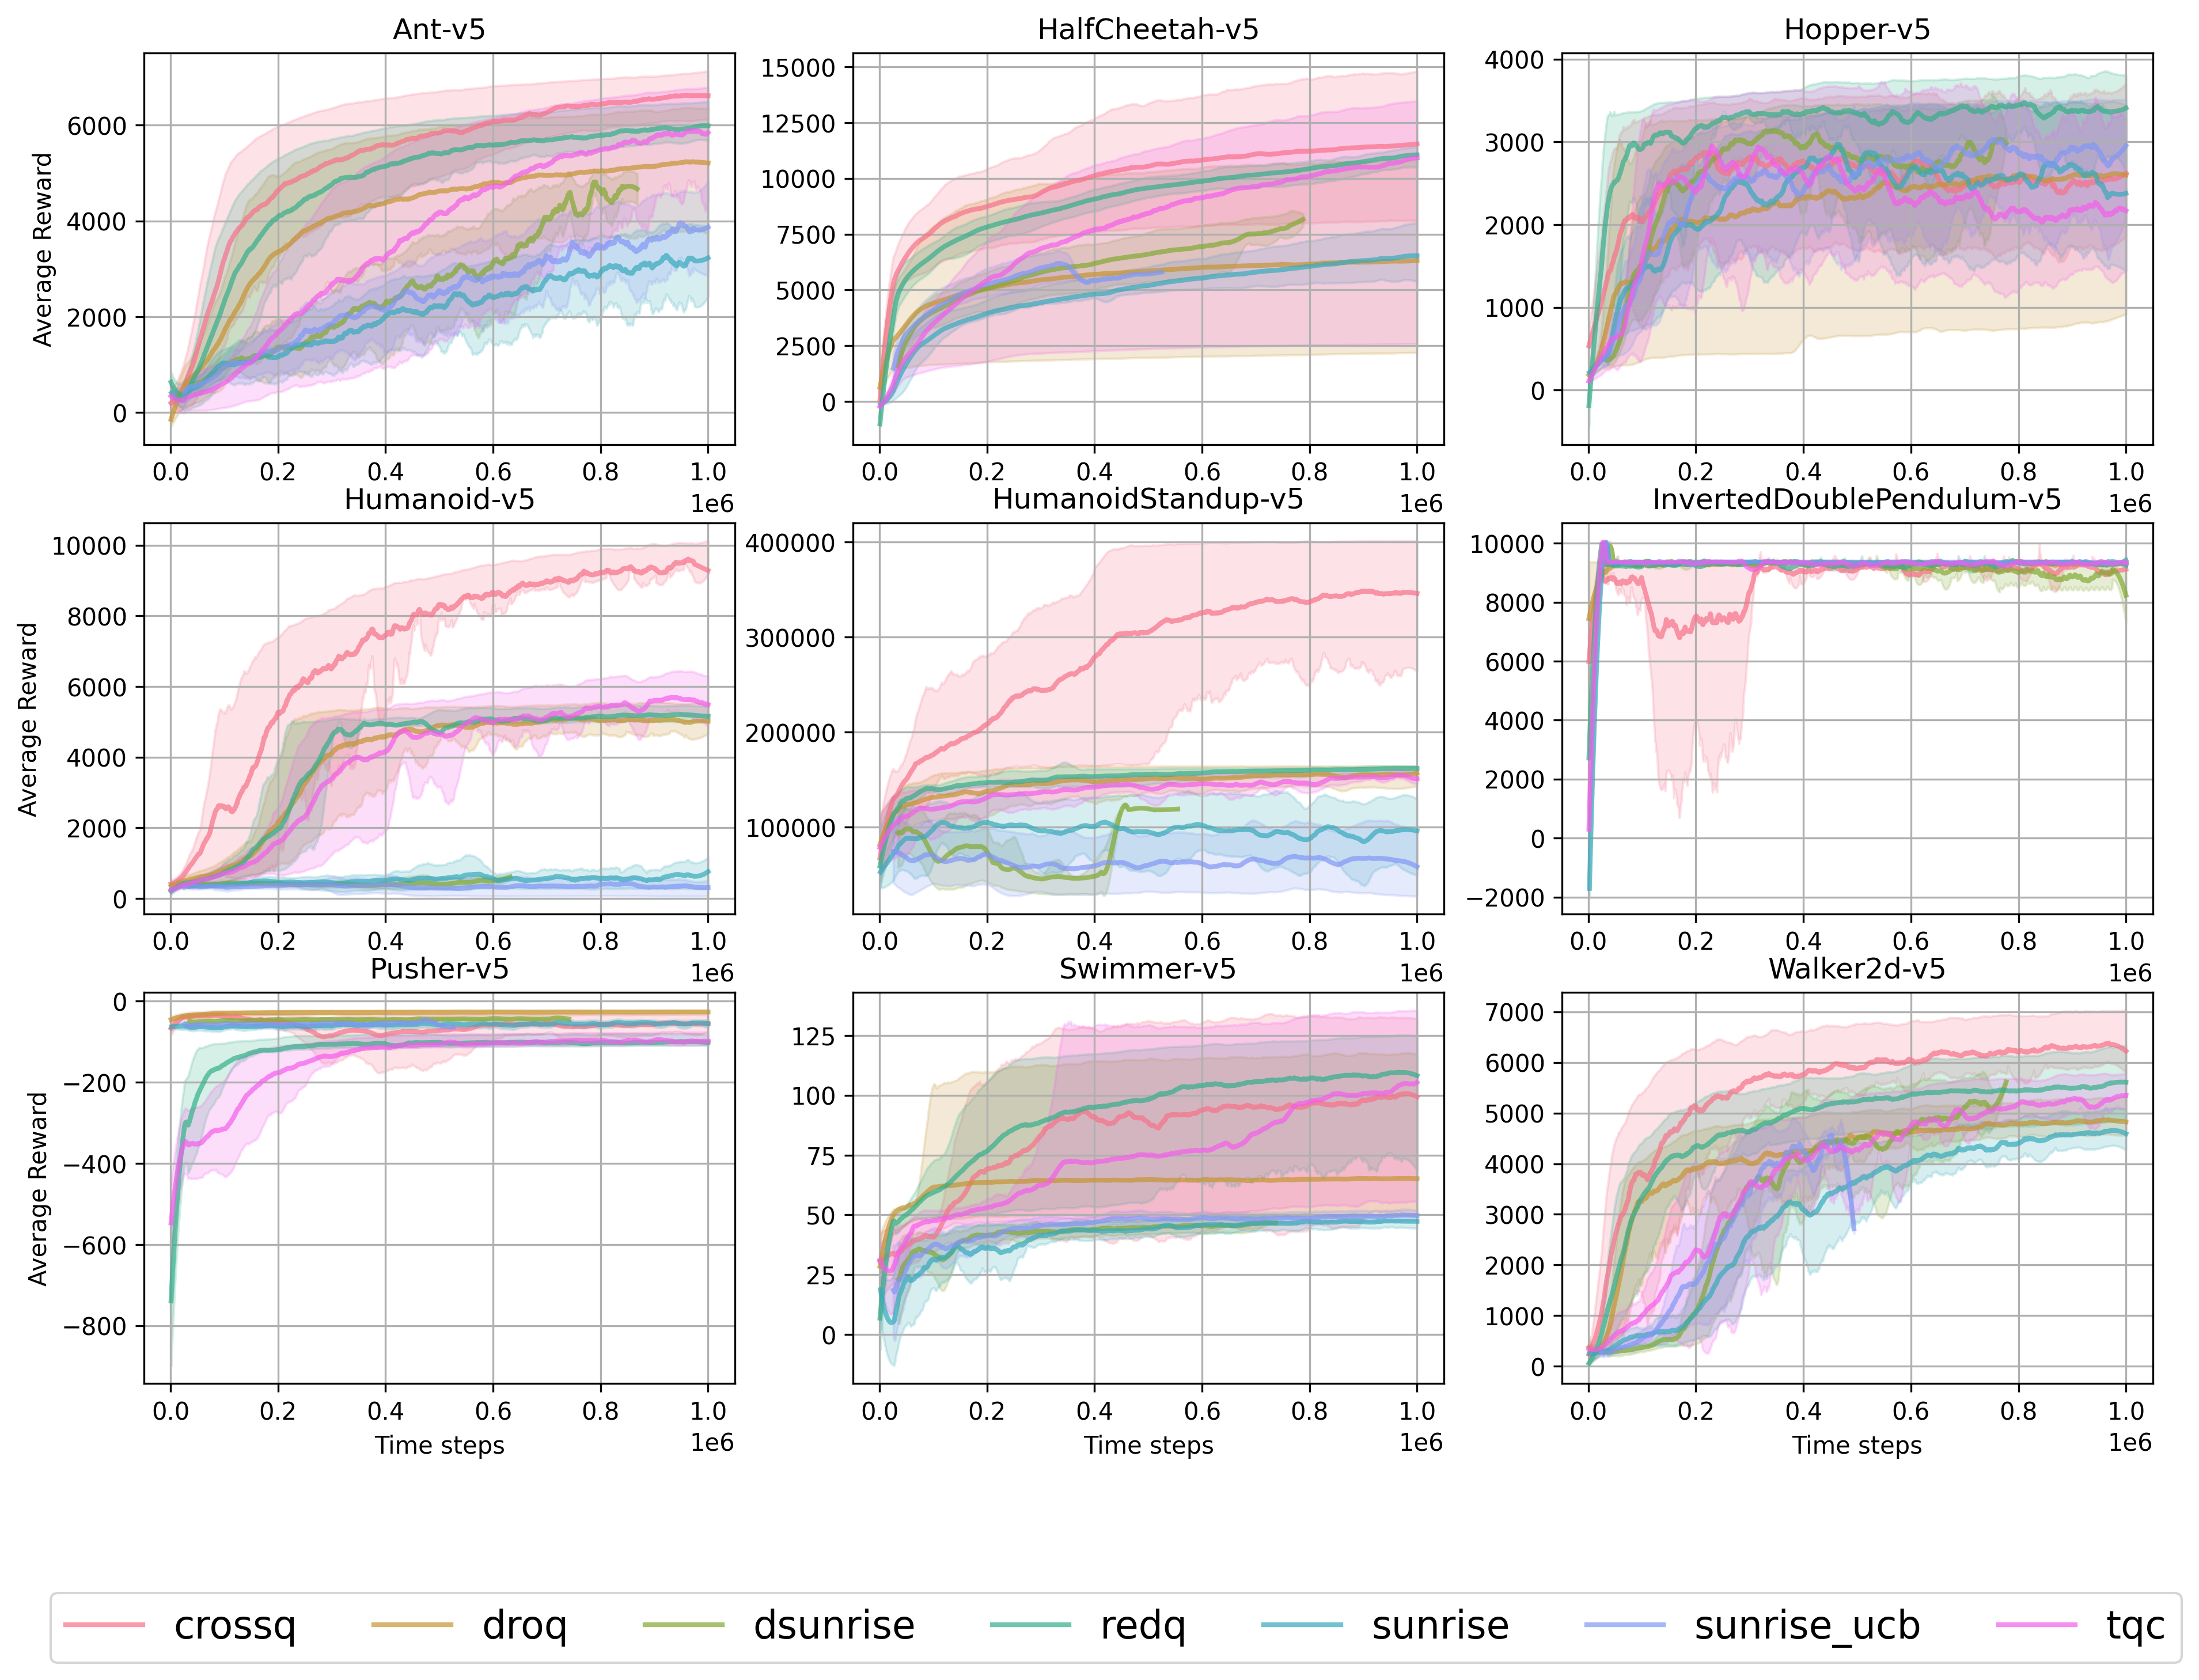
\includegraphics[width=\textwidth]{figures/modern_results.png}
    \caption{Sample Efficiency of the modern algorithms. The line is a smoothed average return across the 100 episodes made by each seed every 1000 times steps. The shaded area is a smoothed 70\% confidence interval highlighted. Note that DSunrise experiments were not completed to 1 million steps, therefore their lines end at the last step completed.}
    \label{fig:sample_efficiency_modern}
\end{figure}

Information on the implementations of the algorithms and the hyperparameters can be found in appendix \ref{C:appendixA}. We see across the algorithms that the newer algorithms outperform the older algorithms in both sample efficiency (how steep the line is) and asymptotic performance (the maximum value of the line). It can be be seen that REDQ and TQC both outperform SAC even though they have the same foundations.

We can see that the newest algorithms are performing the best. Particularly CrossQ performs very well on the more complex environments like \texttt{Humanoid} and \texttt{HumanoidStandup}. It is also observed that CrossQ variance is a lot larger than the other algorithms which is most stark in the \texttt{HumanoidStandup} environment. This is likely due to the fact that CrossQ uses layer normalization which can lead to more variance in the learning process.

The older algorithms perform particularly poorly on the more complex environments like \texttt{Humanoid} and \texttt{HumanoidStandup}. Sunrise which is a ensemble of SAC agents also performs poorly on these environments. Sadly DSunrise also performs poorly on these environments which is understandable given that the base learning algorithm performs poorly. It is conceivable that future work could be done to switch the base algorithm to be CrossQ and use the stability of the ensemble to stabilize the learning process of CrossQ.

\subsection{Computational Efficiency}

The measure of computational efficiency is about measuring the amount of computation it takes to get a an agent to learn a certain task. As there is a variety of different algorithms the most general method is to measure the wall clock time it takes the algorithm to complete a certain number of environment steps.

\begin{figure}[H]
    \centering
    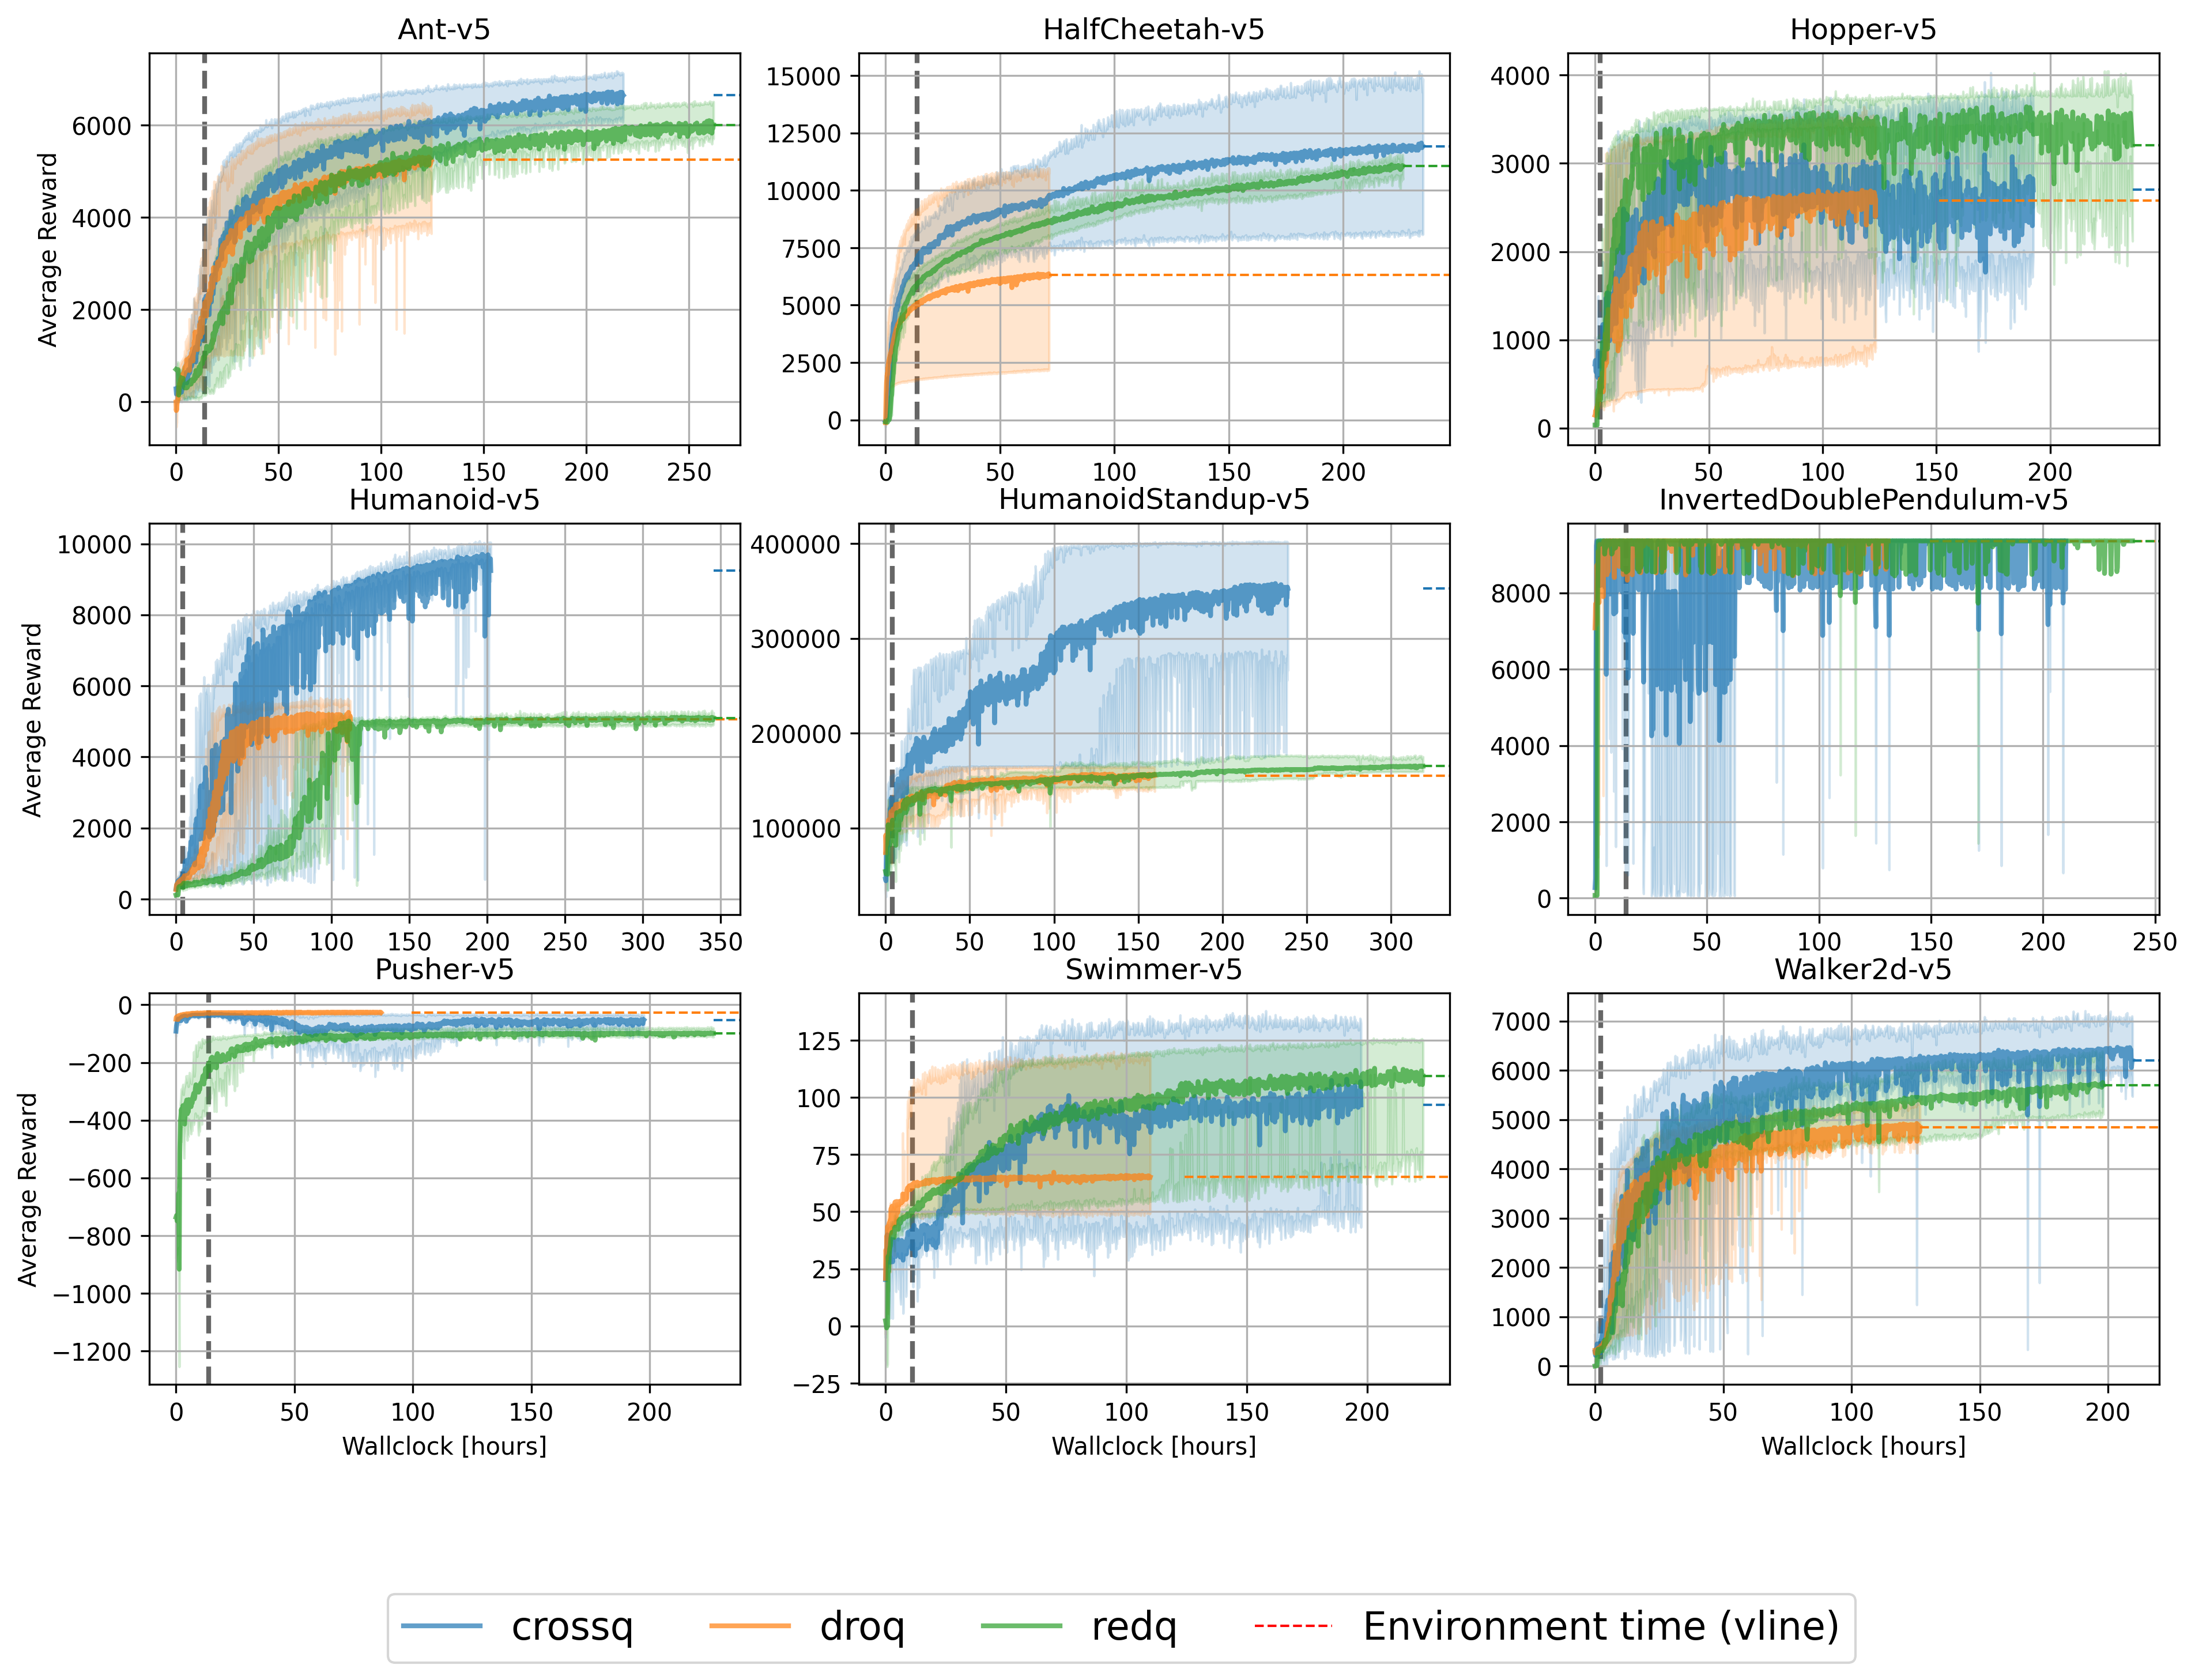
\includegraphics[width=1\textwidth]{figures/wall_clock_results.png}
    \caption{Wall clock time to get to 1 million environment time steps. Vertical lines is how long a million time-steps is in the environment. Horizontal line is the mean average reward at the end of the million steps of learning to help comparisons.}
    \label{fig:computational_efficiency}
\end{figure}


All of experiments were run on similar CPU only machines. See the appendix \ref{C:appendixA} for more information. The goal of graph is not to look at absolute time (however that is interesting to know) it is about the comparing the difference between algorithms given the same hardware. DSunrise is not included in this graph due to the fact that 1 million environment steps of training was not completed by the deadline of this report. Extrapolating from about 500,000 steps suggests that it would take about 250 hours to complete 1 million steps on the hardest environment \texttt{HumanoidStandup}. 

It is interesting to note that the most modern algorithms REDQ and CrossQ are the longest running in terms of wall clock time. More importantly we can see that the method of REDQ having a lot of critics is computationally expensive and results in a wall clock time almost 4 times that of Sunrise which is also a modern ensemble method. This is due to the recent research focus on sample efficiency over computational efficiency.

Looking at the horizontal lines can give us a rough idea of whether we are learning in realtime, faster than realtime or slower than realtime. Importantly we can note that each experiments was run using minimal hardware that is within reach of small Single board computers such as a Raspberry Pi 5.We can see that for a more complicated task like \texttt{HumanoidStandup} we are learning significantly slower than realtime. Whereas the simpler environments are not so drastically slower than realtime. Given the hyperparameters are the same for all environments the only difference in environments is the action and state dimension as well as simulation time. Deeper analysis would have to be done to detangle the affect of simulation time and the action/state dimension in the wall clock time.

\section{Ensemble diversity}
The key idea of DSunrise is to ensure that the diversity of the ensemble of actors is maintained. As DSunrise can be directly compared to Sunrise, we can look at the diversity of the ensemble throughout training.

\begin{figure}
    \centering
    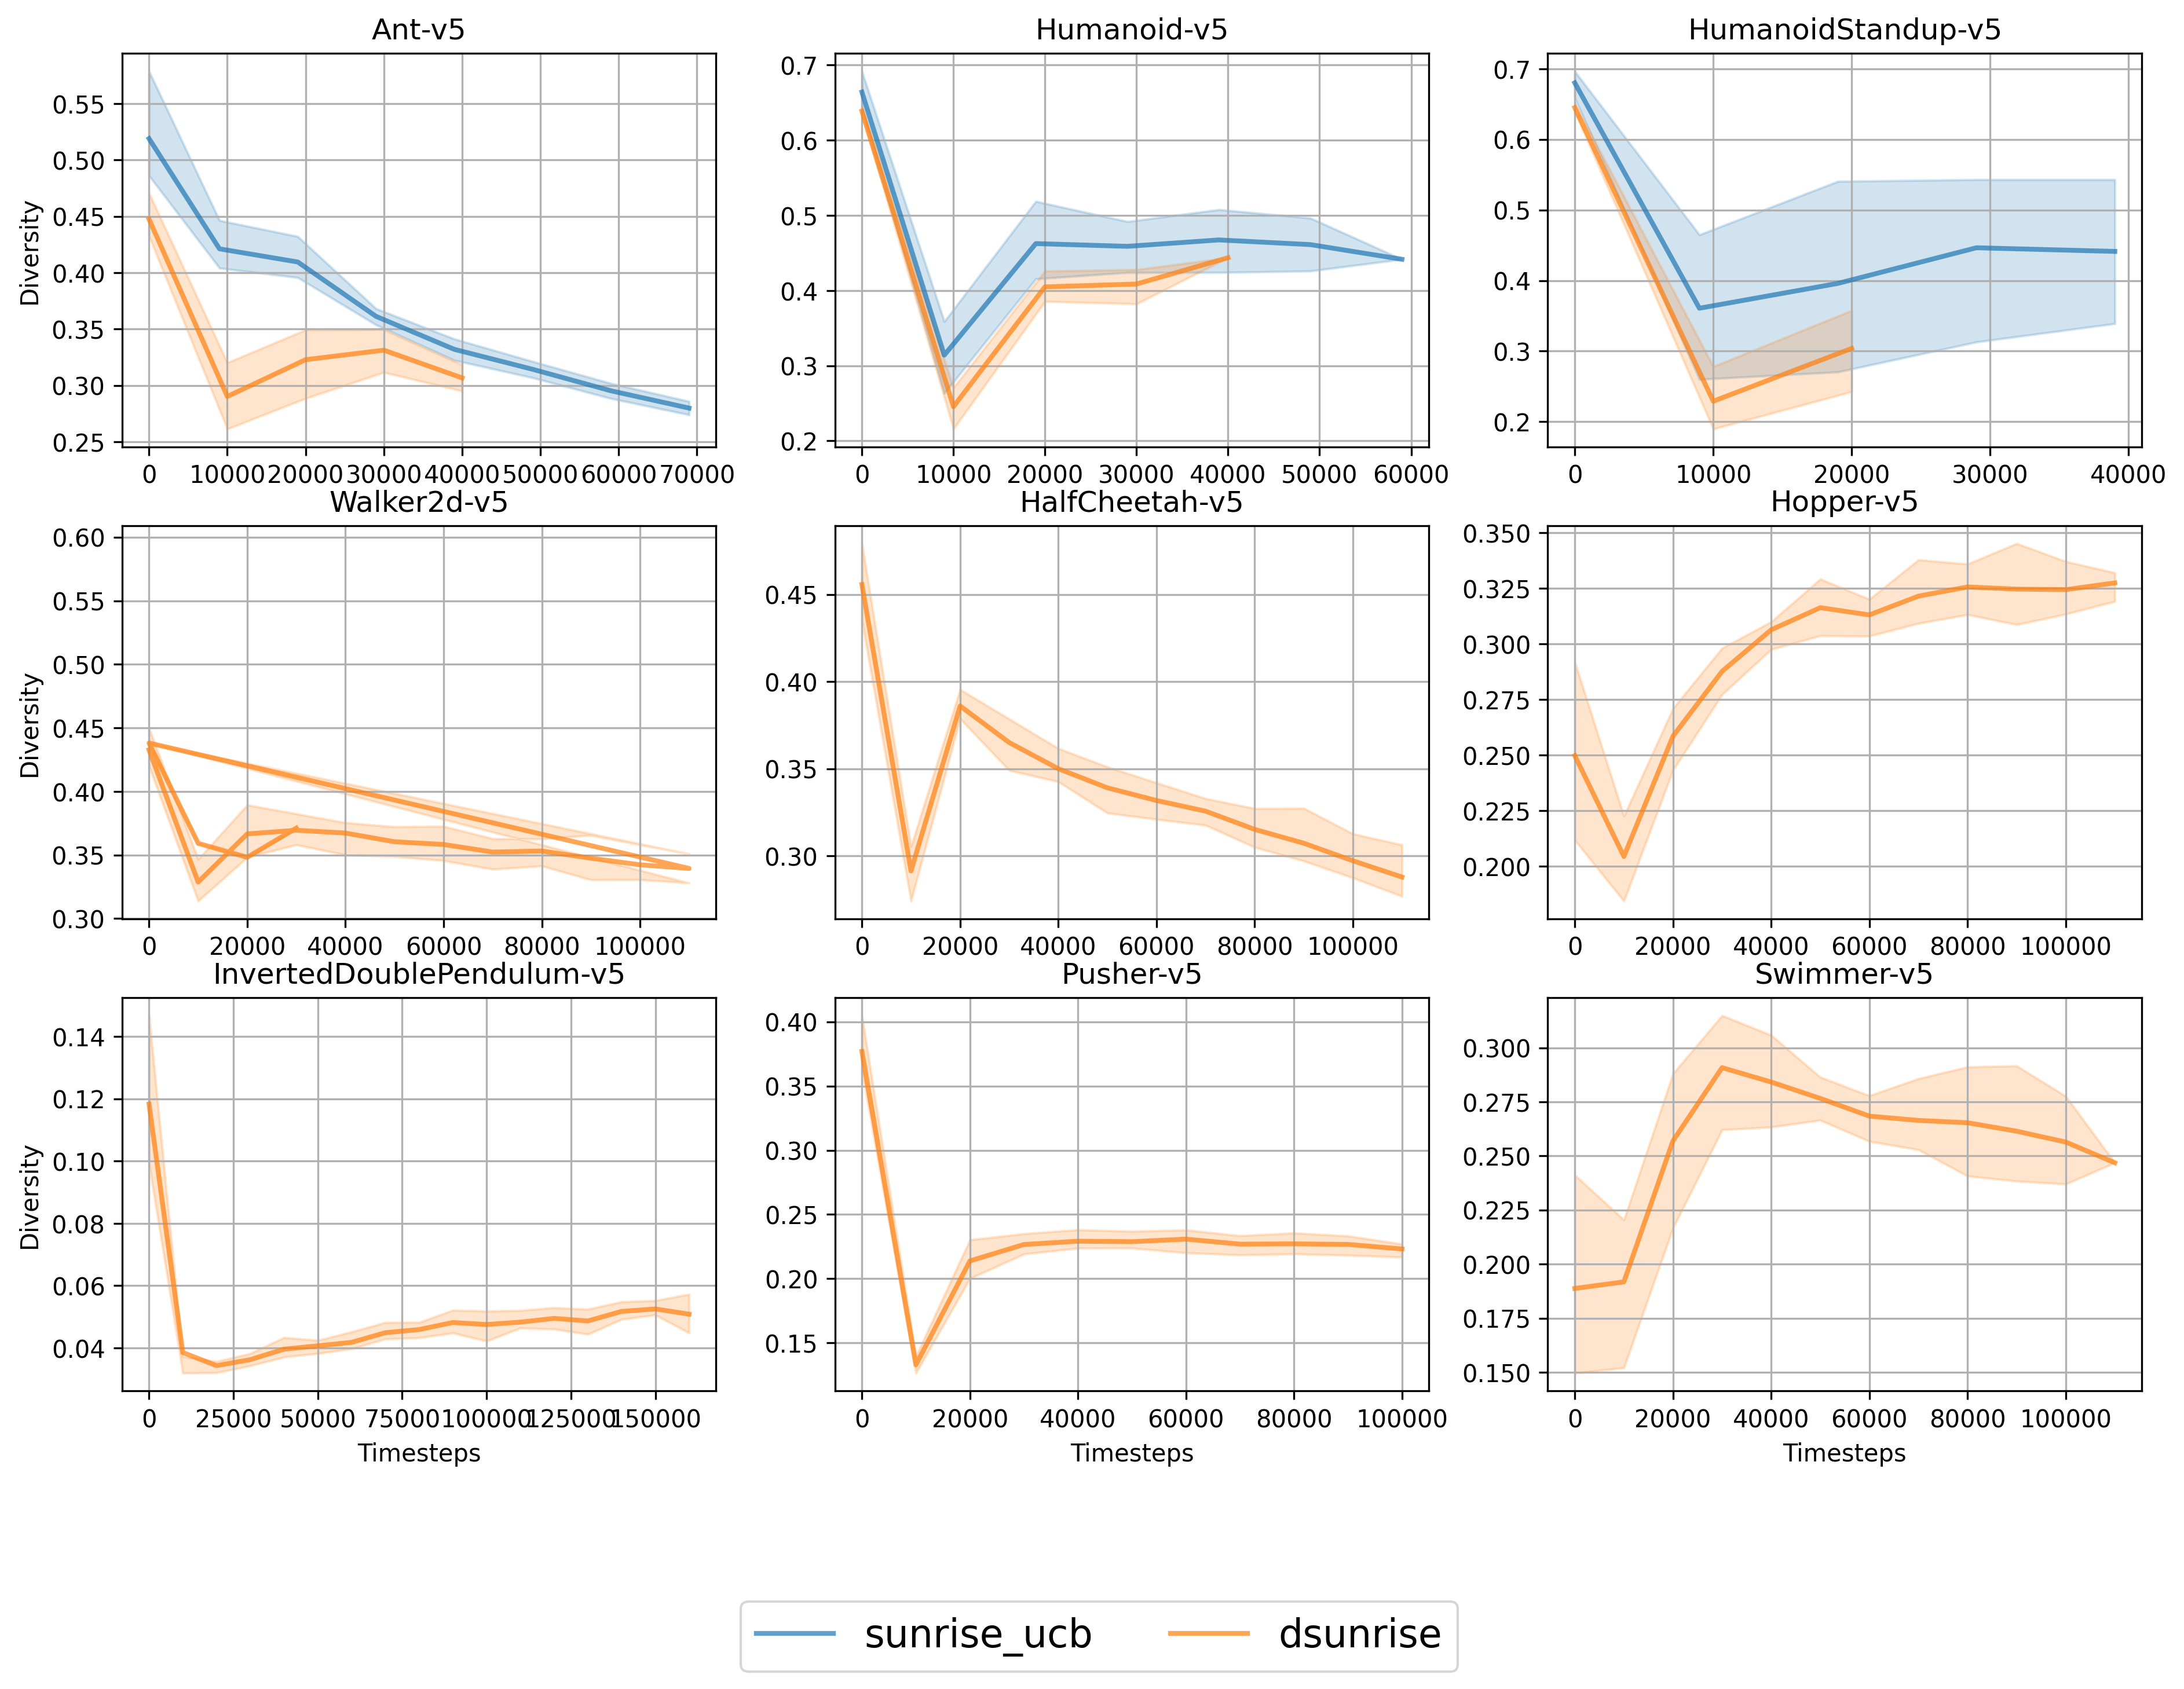
\includegraphics[width=1\textwidth]{figures/diversity_results.png}
    \caption{Diversity of the ensemble over time. The shaded area is a smoothed 70\% confidence interval highlighted.}
    \label{fig:diversity}
\end{figure}

As one would expect the diversity of the ensemble decreases over time as the agents learn to do the task and converge towards the optimal policy. The goal of DSunrise is to maintain the diversity of the ensemble. It is maintaining this diversity by dynamically mutating the ensemble. We  can observe that interestingly the diversity of the ensemble on average is the same as Sunrise which suggests that the dynamic mutation of the ensemble is not having a significant effect on the diversity of the ensemble. As mentioned in further work minimal hyperparameter tuning was done on the mutation parameters.

Looking at different environments we can see different scales of diversity. It is roughly correlated with the complexity of the environment and how well the agent learns. Because the agent never learns in the \texttt{Humanoid} and \texttt{HumanoidStandup} environments they have a consistent diversity that is quite high (almost random). Furthermore as the environments have different action dimensions the diversity metric is not directly comparable. The normalization using max l2 norm means that the diversity is relative to the maximum possible diversity of the action space. Yet larger action spaces will have more ways in which to diverge. The current method of a fixed threshold across all environments and all timesteps may not be the best way to measure diversity.

The environments that learn until convergence like Pusher and InvertedDDoublePendulum have lower diversities. With an interesting phenomenon that the diversity of InvertedDoublePendulum gets higher and much more variable post convergence. Which could be the effect of the mutation slowly "eating" away at the the learned policy. As retrain steps was zero for these experiments one could expect that a small amount of retraining would remove this increase in variability.

\subsection{Changing the ensemble}

In these experiments the removal check was conducted every 10,000 steps. It had 3 outcomes

\begin{itemize}
    \item The ensemble was not changed
    \item An actor was removed from the ensemble
    \item An actor was mutated
\end{itemize}

The removal of actors from the ensemble is not designed to help with learning but instead to reduce the computational cost of the algorithm. In the experiments it was observed that the removal of actors almost never took place as the ensemble never converged enough to a similar policy. The reason could be that the agents were not converging on the optimal policy (likely), the mutation was too strong and without any retraining the policy was different enough (likely), or that the diversity measure was not sensitive enough (plausible). 

\begin{table}[H]
    \centering
    \begin{tabular}{lr}
        \toprule
        env & prob of replacement \\
        \midrule
        Ant-v5 & 0.08 \\
        HalfCheetah-v5 & 0.08 \\
        Hopper-v5 & 0.01 \\
        Humanoid-v5 & 0.00 \\
        HumanoidStandup-v5 & 0.01 \\
        InvertedDoublePendulum-v5 & 0.20 \\
        Pusher-v5 & 0.12 \\
        Swimmer-v5 & 0.12 \\
        Walker2d-v5 & 0.00 \\
        \bottomrule
    \end{tabular}
    \caption{Percent of checks that resulted in a replacement of an actor.}
    \label{tab:avg_replacement_per_check}
\end{table}

As seen in table \ref{tab:avg_replacement_per_check} the average probability of a replacement is low but not negligible. It is interesting to observe that the more complex environments have fewer replacements than the simpler environments. It is reasonable given that the simpler environments are easier to learn and so will converge quicker and once it is near convergence the removal check will always be triggered.

Looking at \ref{fig:diversity} we can see that the diversity of the \texttt{InvertedDoublePendulum-v5} drops below the threshold of 0.2 almost immediately. Whereas the other environments have a diversities well above the threshold. Because \texttt{InvertedDoublePendulum-v5} is below the threshold it will then replace many of the actors in the ensemble.

\begin{figure}
    \centering
    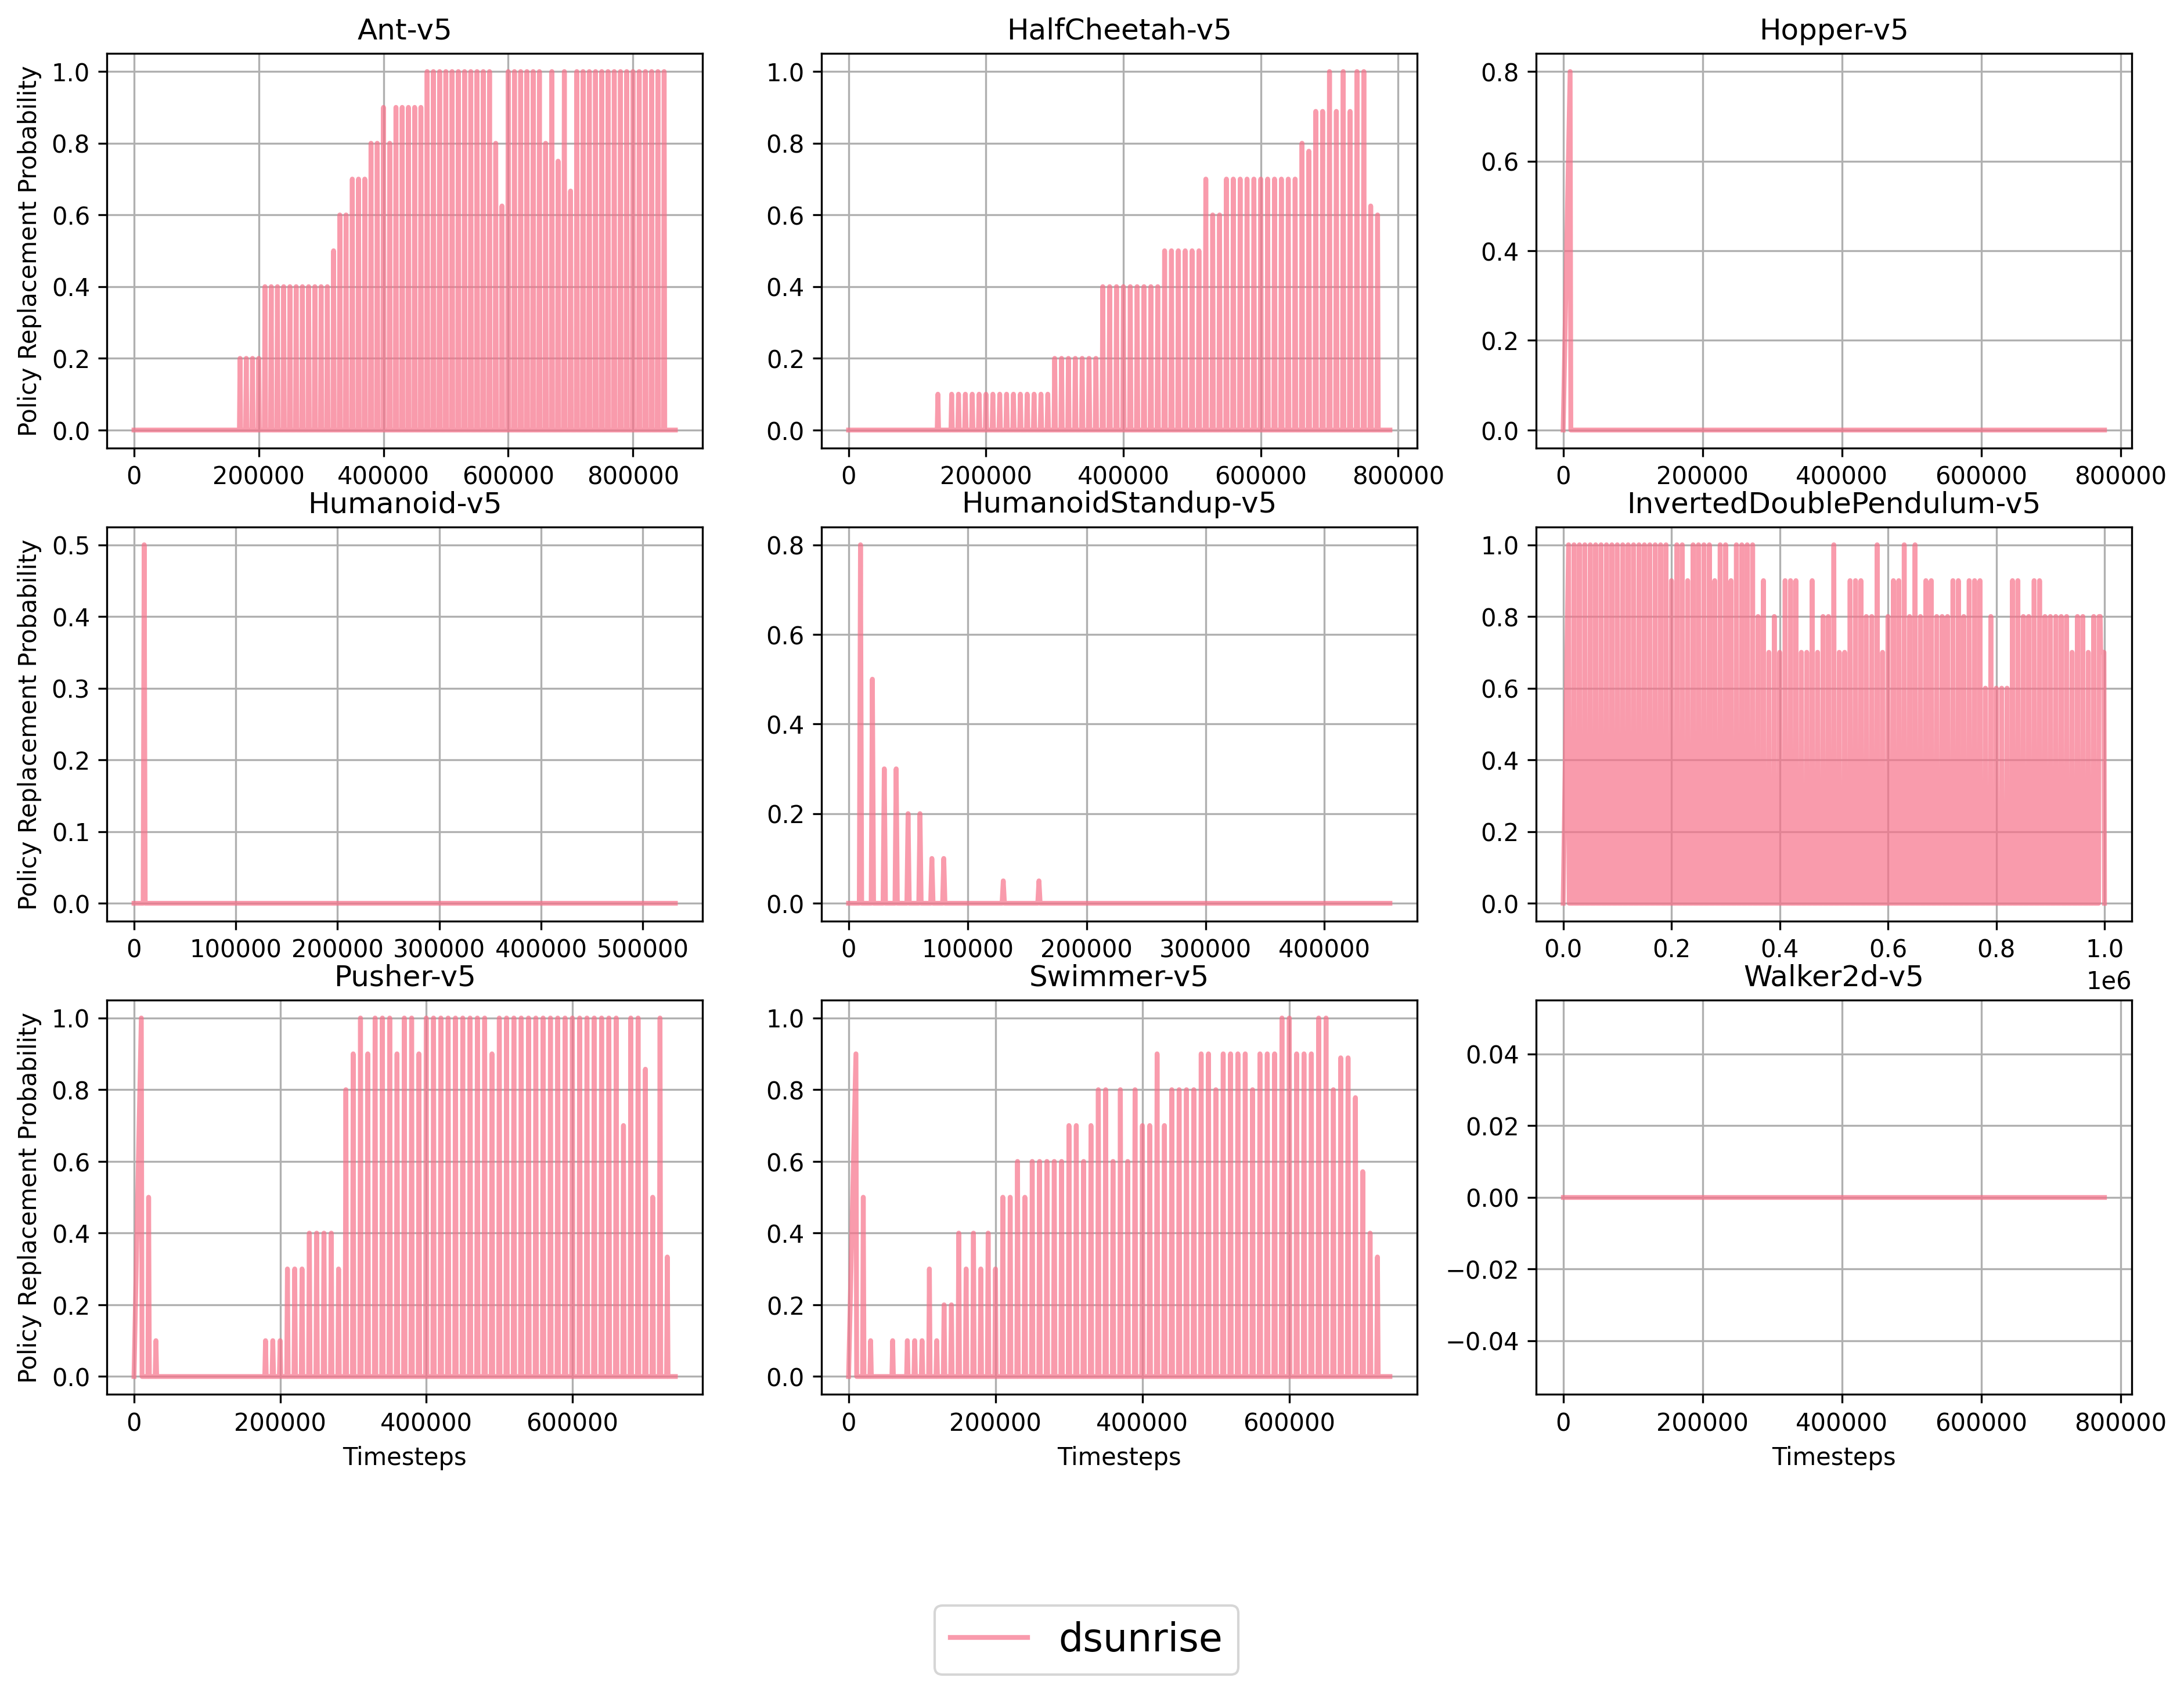
\includegraphics[width=0.8\textwidth]{figures/dsunrise_policy_replacement_probability.png}
    \caption{Ensemble replacement over time. Not the most rigoruos as there are only 10 seeds to average over.}
    \label{fig:ensemble_replacement}
\end{figure}

As one expects that more replacement will happen as training progresses and policies get closer together. \ref{fig:ensemble_replacement} shows what our expectation are with a few peculiarities. Firstly there are 2 environments that have very low very low replacement rates that also have good performance. These are \texttt{Hopper-v5} and \texttt{Walker2d-v5}. Secondly \texttt{InvertedDoublePendulum-v5} has a very high replacement at the start of training and reduces as the effects of mutation take away its convergence and performance which we can see in \ref{fig:sample_efficiency_modern}.
